\documentclass[11pt]{article} 
\newcommand{\cnum}{CM146}
\newcommand{\ced}{Fall 2018}
\newcommand{\ctitle}[2]{\title{\vspace{-0.5in}\cnum, \ced\\Problem Set #1: #2}}
\usepackage{enumitem}
\newenvironment{solution}{\color{blue}{\bf Solution:}}{}
\usepackage[usenames,dvipsnames,svgnames,table,hyperref]{xcolor}
\usepackage{amsmath}
\usepackage{geometry}
\usepackage{graphicx}
\usepackage{subcaption}

\renewcommand*{\theenumi}{\alph{enumi}}
\renewcommand*\labelenumi{(\theenumi)}
\renewcommand*{\theenumii}{\roman{enumii}}
\renewcommand*\labelenumii{\theenumii.}


\begin{document}
% these show up on first page for some reason
\ctitle{1}{Decision trees and k-Nearest Neighbors}
\author{Rodrigo Valle}
\date{29 October 2018}
\maketitle

\section{Problem 1: Splitting Heuristic for Decision Trees}
\begin{solution}
  Please check CCLE to see answer for this question.
\end{solution}

\newpage
\section{Problem 2: Entropy and Information}
\begin{enumerate}
\item Problem 2a

\begin{solution}
  \[IG(S,X_j) = \mathrm{H}(S) - \mathrm{H}(S|X_j)\]
  where $S$ is the set of our training examples and $X_j$ is the attribute that
  we're splitting on.
  
  Also given: our examples $S$ are drawn from a Bernoulli random variable, with
  $p$ positive and $n$ negative examples. Its entropy is given as:
  \[B(q) = -q \log q - (1-q) \log (1-q)\]

  And the entropy of $S$ is given as:
  \[H(S) = B\bigg(\frac{p}{p+n}\bigg)\]

  Given that attribute $X_j$ splits $S$ into $k$ disjoint subsets
  $S_k$, with $p_k$ positive and $n_k$ negative each, we see that splitting on
  $X_j$ gives information gain as follows:
  \[
    IG(S,X_j) = B\bigg(\frac{p}{p+n}\bigg) - \sum_{v \in vals(X_j)} \Pr(v)
    \mathrm{H}(S_k)
  \]

  $H(S|X_j)$, or the conditional entropy, is the sum of the entropies of the
  subsets formed after the split, weighted by the probability that attribute
  $X_j = v$.

  Plugging in $\Pr(v) = \frac{p_k + n_k}{p + n}$, we have
  \begin{align*}
    IG(S,X_j) &= B\bigg(\frac{p}{p+n}\bigg) - \frac{p_k + n_k}{p + n}
    \sum_{v \in vals(X_j)} \mathrm{H}(S_k)\\
    IG(S,X_j) &= B\bigg(\frac{p}{p+n}\bigg) - k\frac{p_k + n_k}{p + n}
    \mathrm{H}(S_k)\\
  \end{align*}
  noting that $k(p_k+n_k) = p + n$ follows from the given information, we
  simplify further:
  \begin{align*}
    IG(S,X_j) &= B\bigg(\frac{p}{p+n}\bigg) - \mathrm{H}(S_k)\\
    IG(S,X_j) &= B\bigg(\frac{p}{p+n}\bigg) - B\bigg(\frac{p_k}{p_k+n_k}\bigg)
  \end{align*}

  Now we argue that $B\bigg(\frac{p}{p+n}\bigg) = B\bigg(\frac{p_k}{p_k+n_k}\bigg)$
  because $\frac{p}{p+n} = \frac{p_k}{p_k + n_k}$. We have that there are $k$
  disjoint subsets of $S$ called $S_k$, each with the same $p_k$ and $n_k$ so
  \begin{itemize}
    \item $\sum p_k = p$
    \item $k p_k = p$
  \end{itemize}
  and
  \begin{itemize}
    \item $\sum n_k = n$
    \item $k n_k = n$
  \end{itemize}

  \[
    \frac{p_k}{p_k + n_k} = \frac{kp_k}{kp_k + kn_k} = \frac{p}{p + n}
  \]

  Thus
  \begin{align*}
    IG(S,X_j) &= B\bigg(\frac{p}{p+n}\bigg) - B\bigg(\frac{p_k}{p_k+n_k}\bigg)\\
              &= B\bigg(\frac{p}{p+n}\bigg) - B\bigg(\frac{p}{p+n}\bigg)\\
              &= 0
  \end{align*}

\end{solution}

%\item Problem 1b
\end{enumerate}

\newpage
\section{Problem 3: k-Nearest Neighbors and Cross-validation}
\begin{enumerate}
  \item Problem 3a

  \begin{solution}
  The value $k = 0$ will minimize the training error on this dataset. If a point
  can be its own neighbor, then when given a point from the training set $k = 0$
  will re-select itself from the training set and give the correct label.
  Training error will be zero.
  \end{solution}

  \item Problem 3b

  \begin{solution}
  Using values of $k$ that are too large will result in looking at extra
  points (outliers, almost) that are significantly further away from where
  we're trying to predict, resulting in more misclassifications.\ e.g $k > 7$ on
  a point at say (10, 1) causes us to begin considering the further group of
  points that have (ideally) less relevance, clouding our final prediction.

  Using values of $k$ that are too small can cause K Nearest Neighbors to
  overfit by not considering enough surrounding data to make a prediction that
  will generalize.
  \end{solution}

  \item Problem 3c
    
  \begin{solution}
  Assume L2 norm.
  \begin{itemize}
    \item $k = 1$, 10 wrong out of 14
    \item $k = 3$, 6 wrong out of 14
    \item ANSWER: $k = 5$, 4 wrong out of 14
  \end{itemize}
  \end{solution}
\end{enumerate}

\newpage
\section{Problem 4: Programming exercise}
\begin{itemize}
  \item 4.1 Visualization
  \begin{enumerate}
    \item See Figure~\ref{fig:histograms} below.

      From these plots, we can see
      \begin{itemize}
        \item The only age group more likely to survive than die was in the 0-10
          year range. Those between ages 20-30 were significantly more likely to
          die than live.
        \item Those with at least one parent or child on-board were more likely
          to survive.
        \item Upper-class passengers were more likely to live, middle-class
          passengers had closer to a 50/50 chance, and lower-class passengers
          were significantly more likely to die.
        \item Women were more likely to survive than men.
        \item Those with at least one sibling or spouse on board significantly
          decreased their chances of death.
        \item Those who paid upwards of \$50 for fare had increased chance of
          survival.
        \item Those who embarked at the very beginning of the Titanic's trip had
          increased chances of survival. Others who embarked along the way were
          more likely to perish.
      \end{itemize}
      \newgeometry{textwidth=8in, textheight=11in}
      \begin{figure}
        \centering
        \begin{subfigure}[b]{0.49\textwidth}
          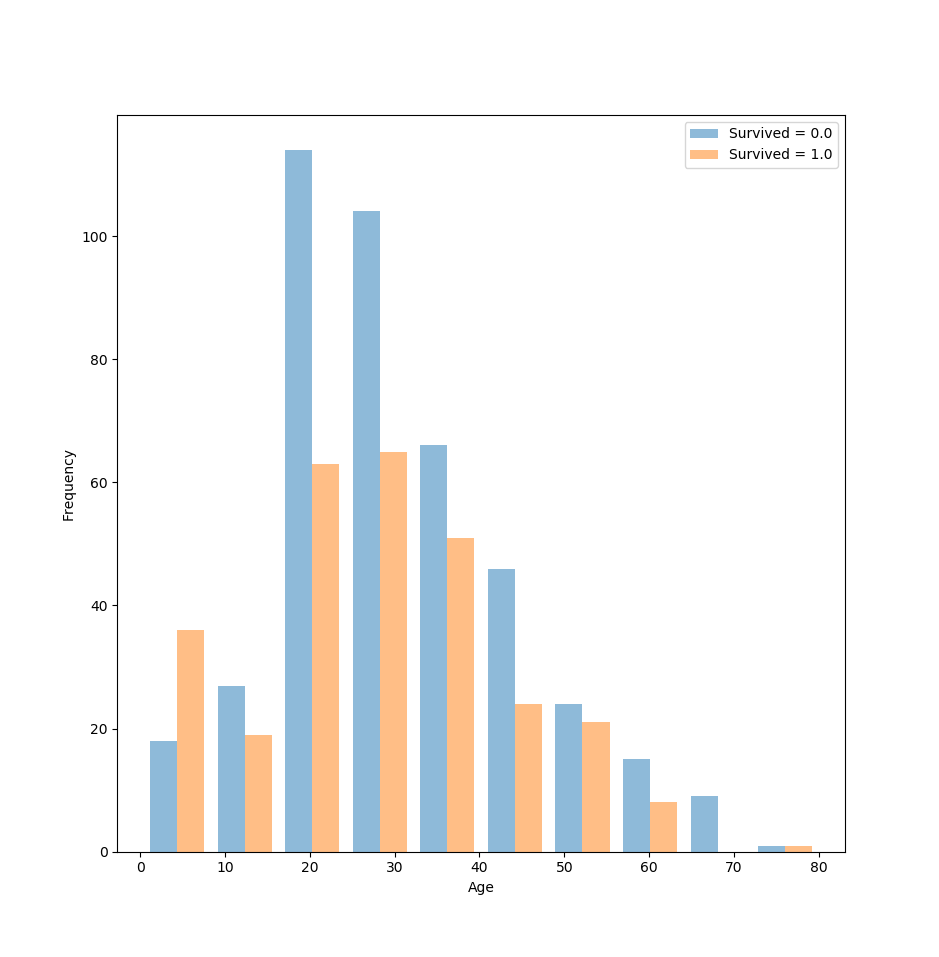
\includegraphics[width=\textwidth]{figs/age.png}
          \caption{Age}
        \end{subfigure}
        %add desired spacing between images, e.g. ~, \quad, \qquad, \hfill etc. 
        %(or a blank line to force the subfigure onto a new line)
        \begin{subfigure}[b]{0.49\textwidth}
          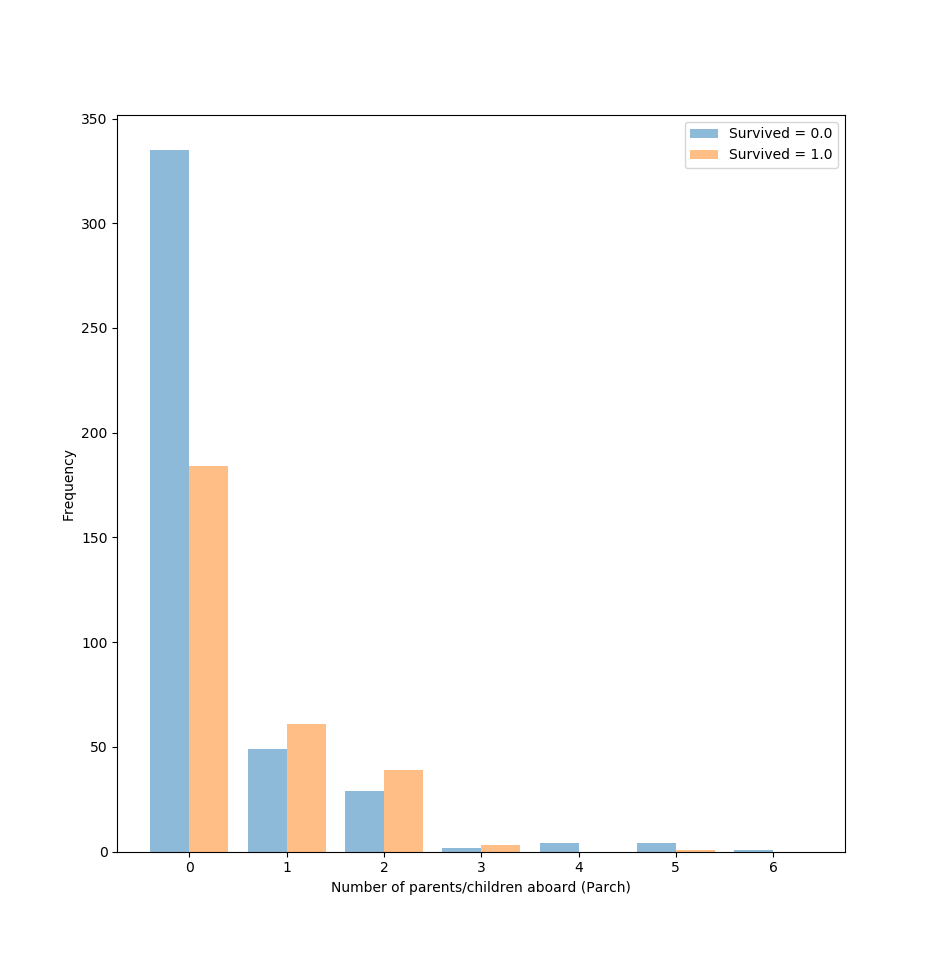
\includegraphics[width=\textwidth]{figs/parch.png}
          \caption{Parch}
        \end{subfigure}

        \begin{subfigure}[b]{0.49\textwidth}
          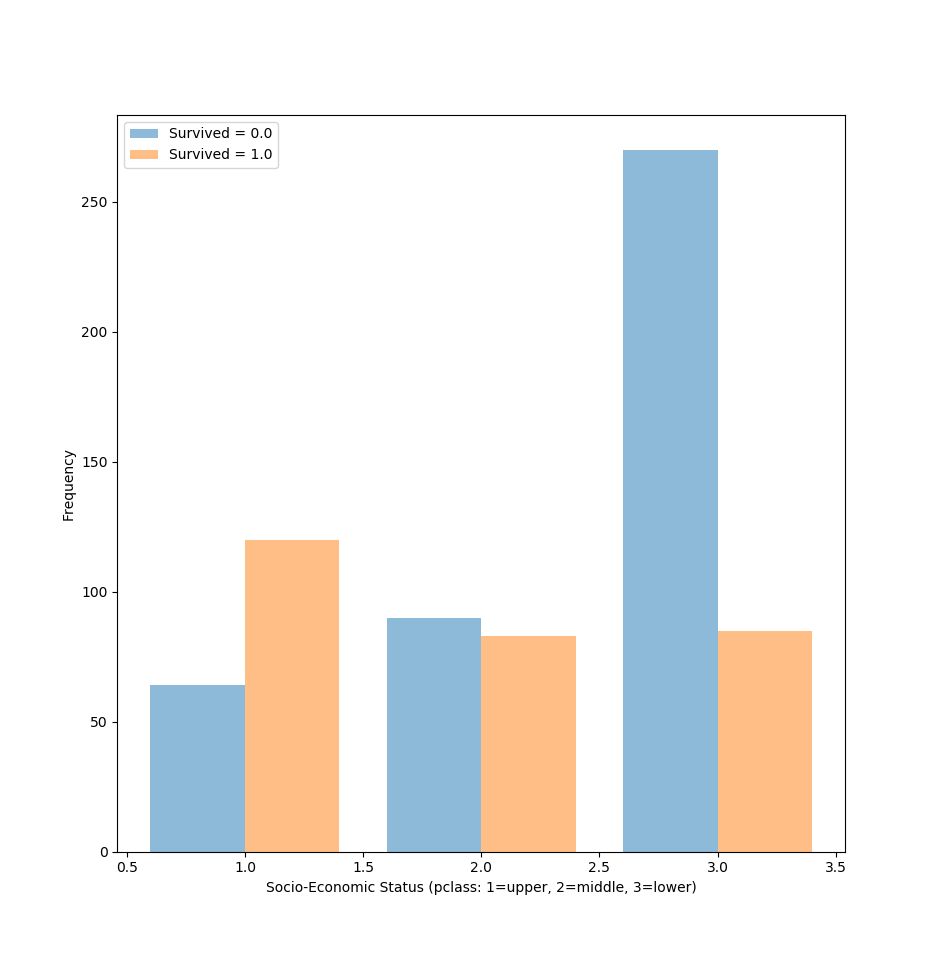
\includegraphics[width=\textwidth]{figs/pclass.png}
          \caption{Pclass}
        \end{subfigure}
        \begin{subfigure}[b]{0.49\textwidth}
          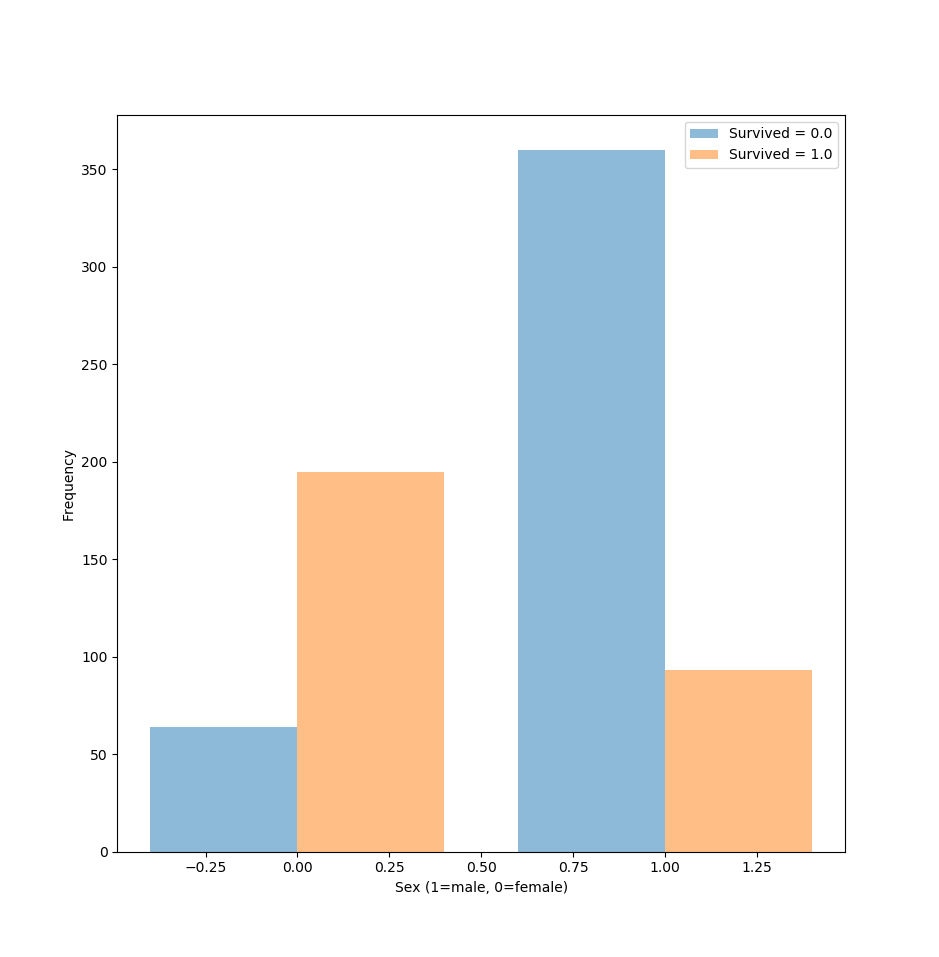
\includegraphics[width=\textwidth]{figs/sex.png}
          \caption{Sex}
        \end{subfigure}
      \end{figure}
      \clearpage
      \begin{figure}
        \ContinuedFloat
        \centering
        \begin{subfigure}[b]{0.49\textwidth}
          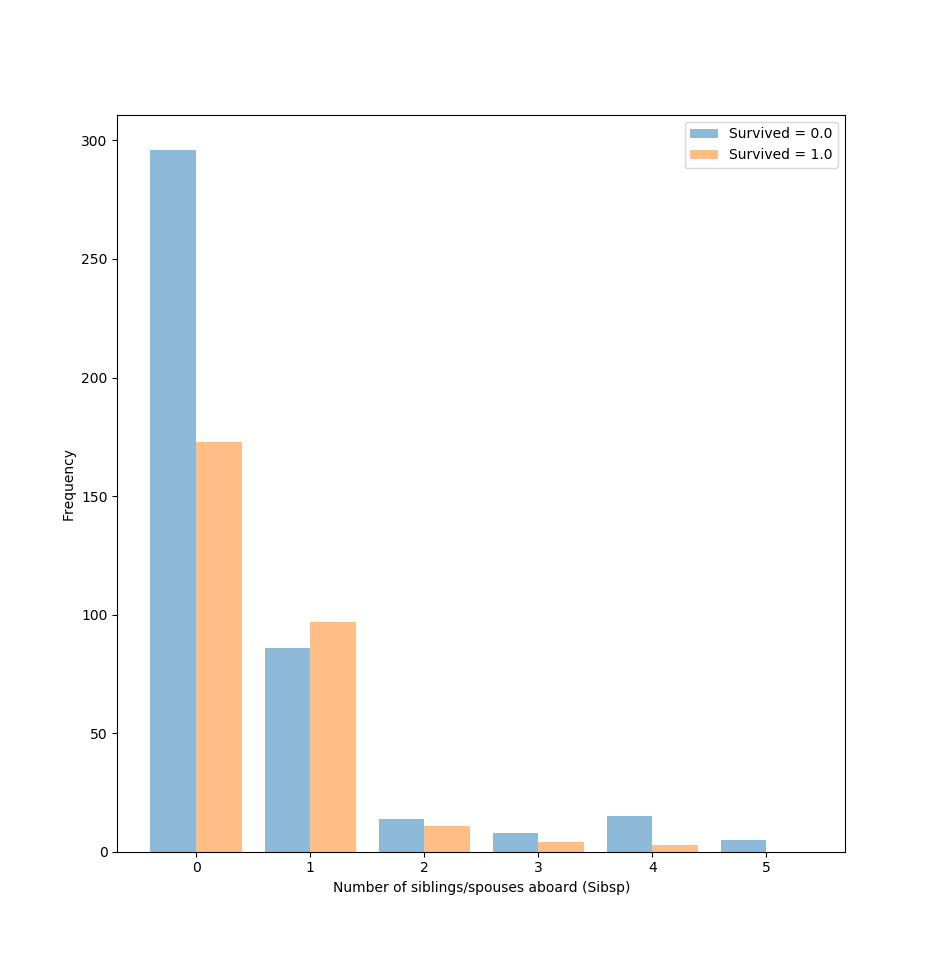
\includegraphics[width=\textwidth]{figs/sibsp.png}
          \caption{Sibsp}
        \end{subfigure}
        \begin{subfigure}[b]{0.49\textwidth}
          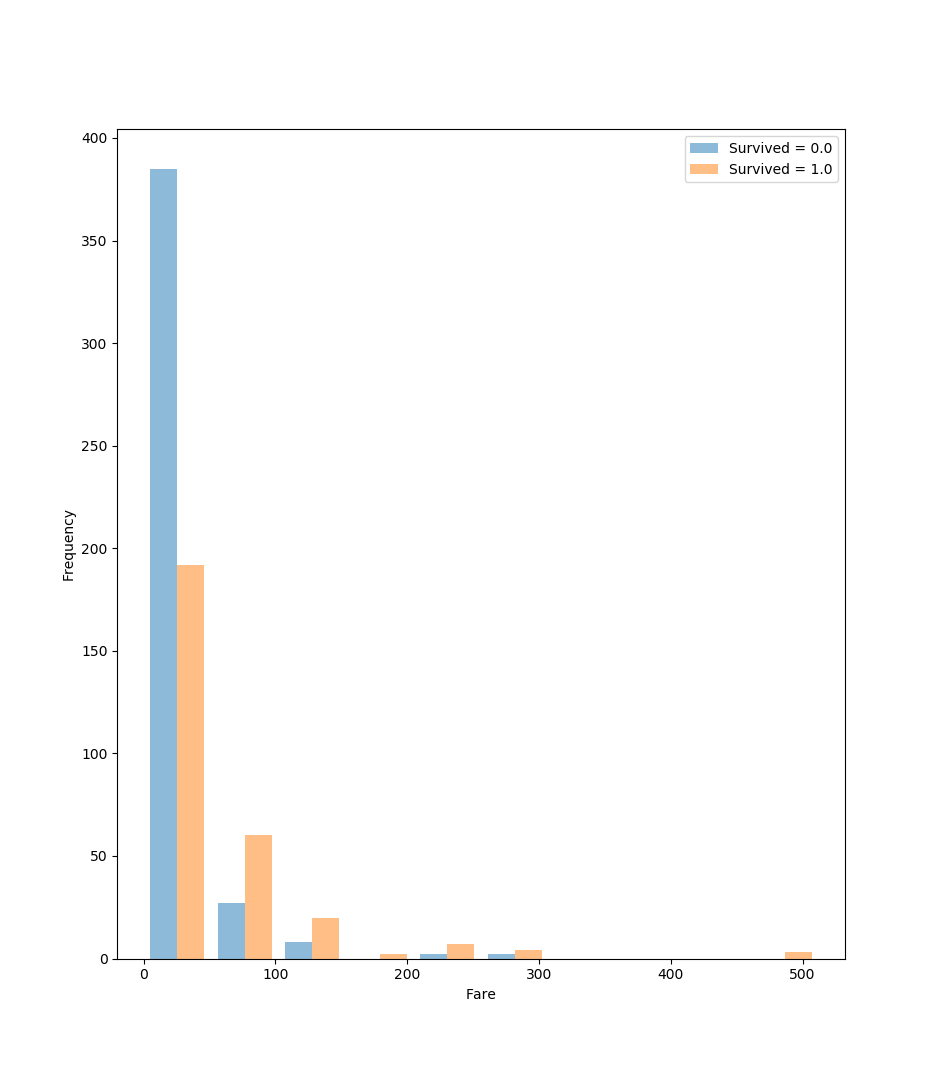
\includegraphics[width=\textwidth]{figs/fare.png}
          \caption{Fare}
        \end{subfigure}

        \begin{subfigure}[b]{0.49\textwidth}
          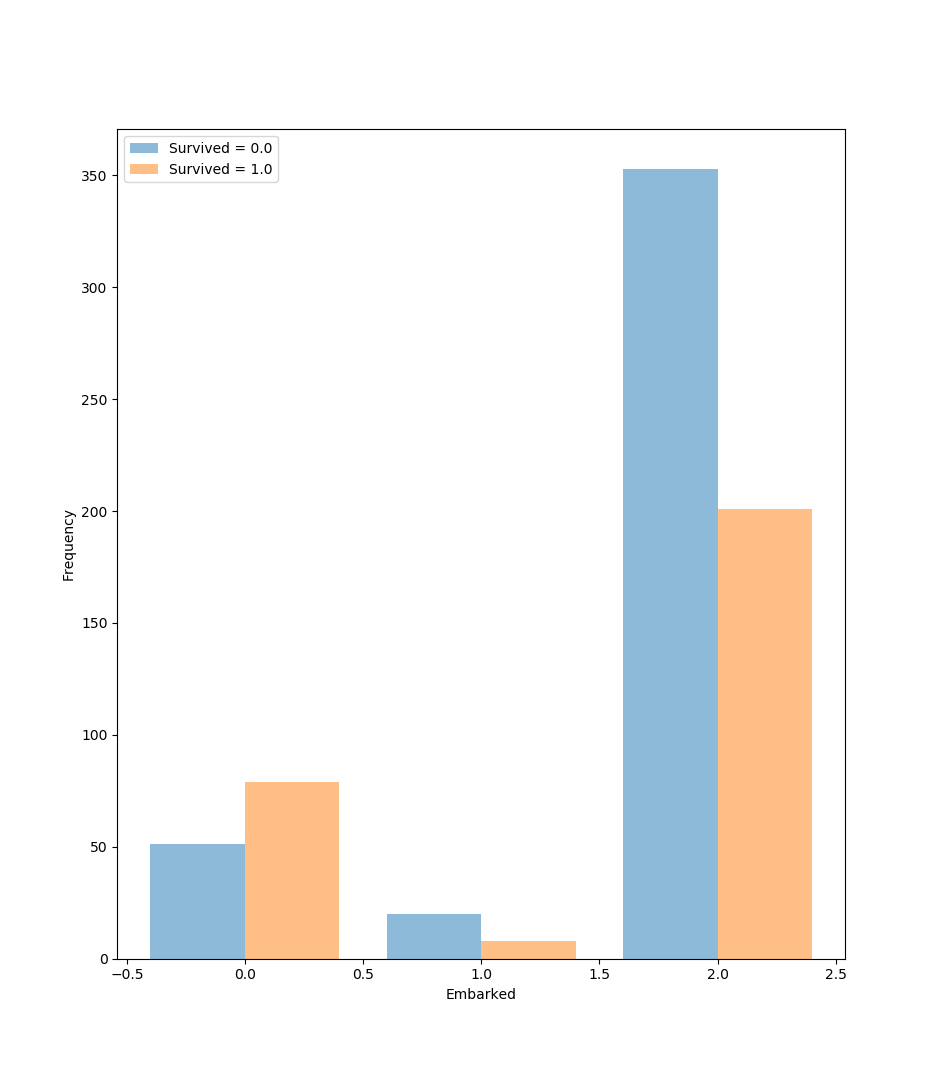
\includegraphics[width=\textwidth]{figs/embarked.png}
          \caption{Fare}
        \end{subfigure}

        \caption{Distributions of all attribute splits}\label{fig:histograms}
      \end{figure}
      \restoregeometry

      \item Implemented \texttt{RandomClassifier}.
      \item Training error of \texttt{DecisionTreeClassifier}: 0.014
      \item Training error of \texttt{KNeighborsClassifier}:
        \begin{itemize}
          \item $k = 3$: 0.167
          \item $k = 5$: 0.201
          \item $k = 7$: 0.240
        \end{itemize}
      \item Average training and test error of each classifier:
        \begin{itemize}
          \item \texttt{MajorityVoteClassifier}
            \begin{itemize}
              \item train: 0.404
              \item test: 0.407
            \end{itemize}
          \item \texttt{RandomClassifier}
            \begin{itemize}
              \item train: 0.486
              \item test: 0.478
            \end{itemize}
          \item \texttt{DecisionTreeClassifier}
            \begin{itemize}
              \item train: 0.012
              \item test: 0.241
            \end{itemize}
          \item \texttt{KNeighborsClassifier}
            \begin{itemize}
              \item train: 0.212
              \item test: 0.315
            \end{itemize}
        \end{itemize}
        
      \item See Figure~\ref{fig:bestk}. Best $k$ was found to be $k=7$.

        Observations: $k=1$ is the worst $k$ we found, clearly looking at more
        data helps us make a better estimate. Around $k=33$ though, we see that
        looking at more data (increasing $k$) starts adding error to our
        estimates --- this is where we've started to consider enough data points
        that are too far away from the point we want to classify that they
        outnumber the closer data points.

      \item See Figure~\ref{fig:bestdepth}. Best depth was found to be depth=3
        (note: depth would change somewhat sporadically between 3 and 6 ---
        cause unknown, could be a floating point hardware/math issue) (even
        better sidenote: switching to a different linux desktop would reliably
        change the result)

        After depth=6, we can observe some overfitting: test error starts going
        up as train error trends down predictably. Our model has become too
        overfitted to the training data set and will perform amazingly well on
        training data that it has seen, but fails to generalize to the test
        data that it hasn't seen.

      \item See Figure~\ref{fig:learning_curve}.
        
        Observations: With K Nearest Neighbors, training error slopes
        predictably downwards, and test error follows suit for the most part
        with some noise --- this means that training KNN with more data causes
        its predictive performance to increase, although not as reliably as we
        would hope.

        With the Decision Tree Classifier, training error starts low and testing
        error high with a small training data set. With more training data, they
        converge to the point where training error closely mirrors test error,
        clearly indicating that increasing the amount of data available to train
        a decision tree will likely increase the quality of the prediction. It
        also showcases the decision tree to learn quickly, with quick
        convergence of training and test error at low fractions of the training
        data.

        \begin{figure}
          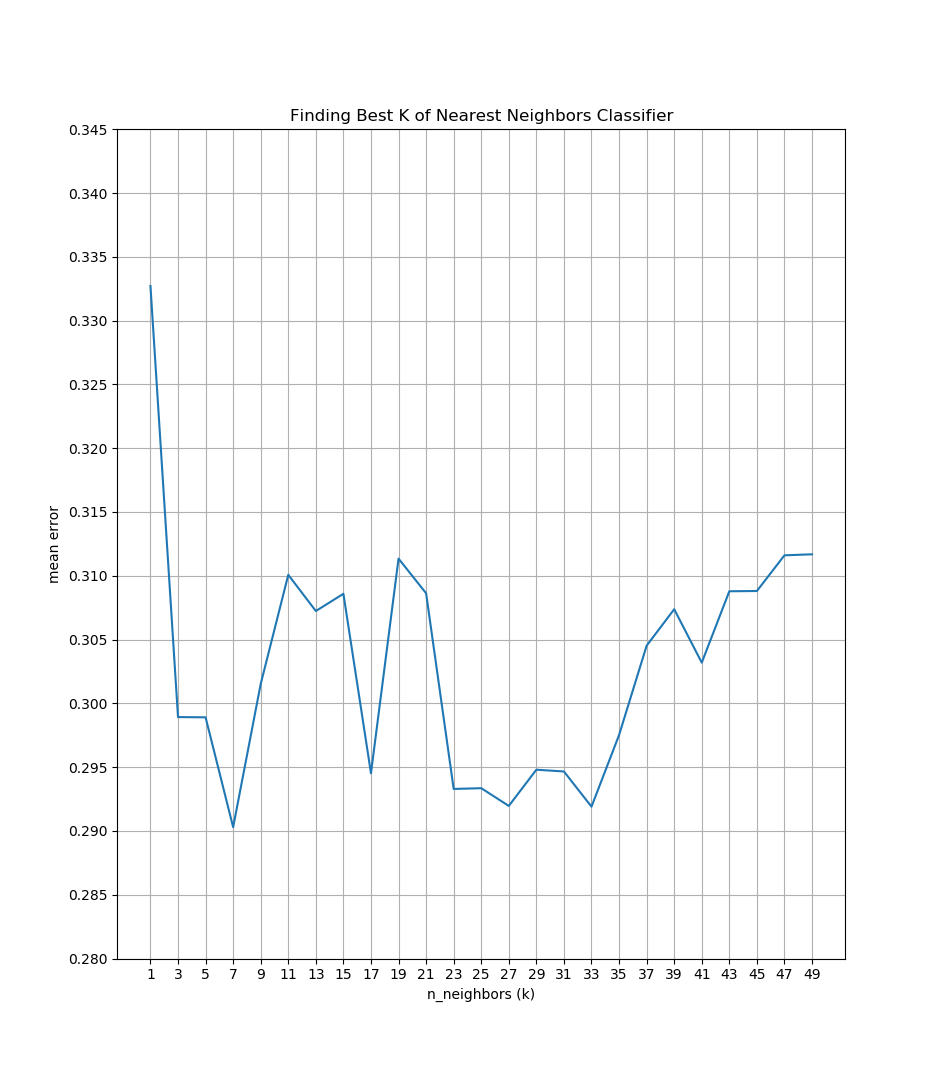
\includegraphics[width=\textwidth]{figs/best_k_odd.png}
          \caption{Best k}
          \label{fig:bestk}
        \end{figure}

        \begin{figure}
          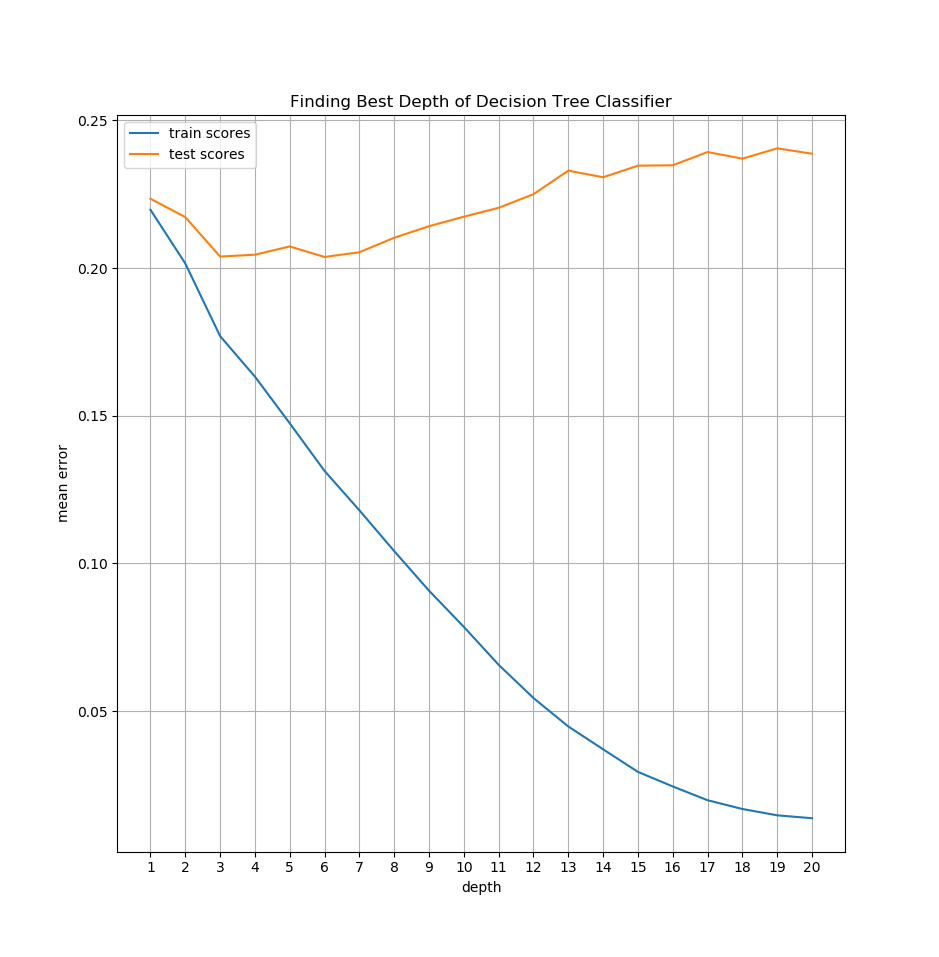
\includegraphics[width=\textwidth]{figs/best_depth_8020split.png}
          \caption{Best depth}
          \label{fig:bestdepth}
        \end{figure}

        \begin{figure}
          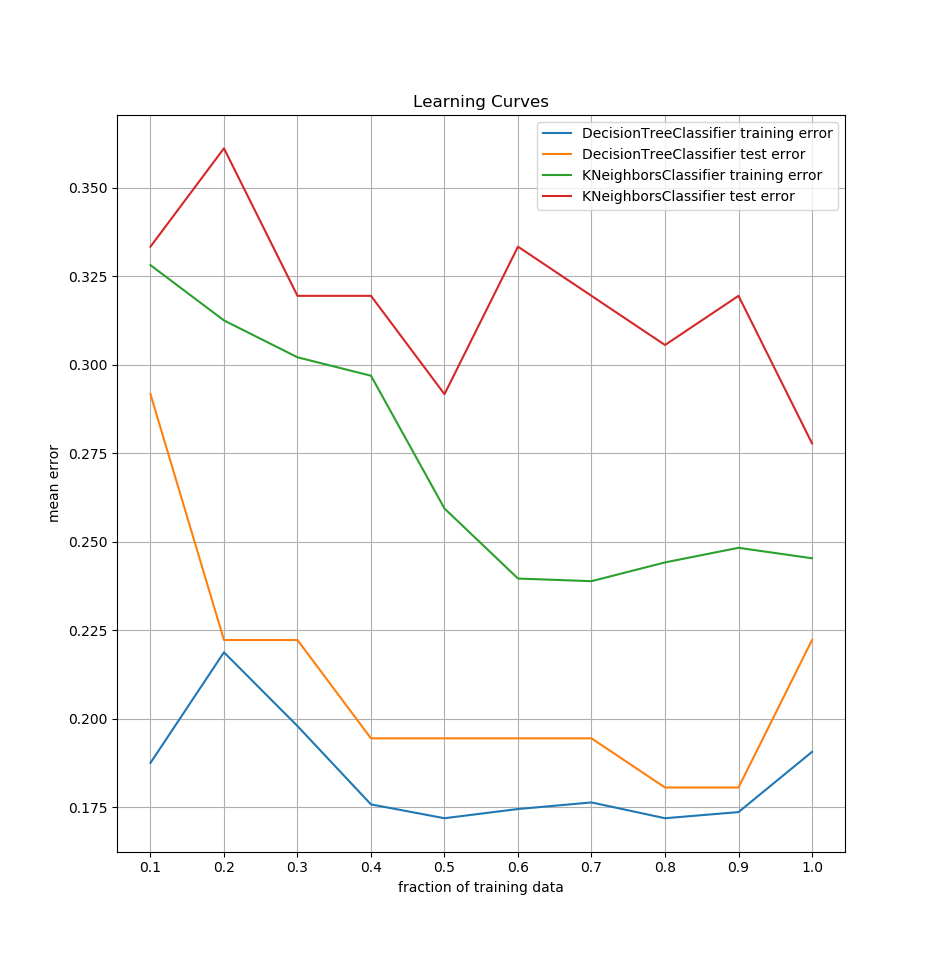
\includegraphics[width=\textwidth]{figs/all_learning_curve.png}
          \caption{Learning Cruves for Decision Tree and K Nearest Neighbors}
          \label{fig:learning_curve}
        \end{figure}
    \end{enumerate}
\end{itemize}
\end{document}
